\documentclass{beamer}
\usepackage[english,francais]{babel}
\usepackage[T1]{fontenc}
\usepackage{lmodern}

%
% Choisir l'apparence de votre pr�sentation.
%
% Pour plus de th�mes, de th�mes de couleur ou de th�me de fontes, cf. :
% http://deic.uab.es/~iblanes/beamer_gallery/index_by_theme.html
%
\mode<presentation>
{
  \usetheme{Warsaw}       % ou essayer Darmstadt, Madrid, Dresden, ...
  \usecolortheme{default} % ou essayer albatross, beaver, crane, ...
  \usefonttheme{default}  % ou essayer serif, structurebold, ...
  \setbeamertemplate{navigation symbols}{}
  \setbeamertemplate{caption}[numbered]
} 

\title{D�dicace du cimeti�re de Gettysburg}
\author{Abraham Lincoln}
\institute{�tats-Unis d'Am�rique}
\date{19 nov. 1863}

\begin{document}

\begin{frame}
  \titlepage
\end{frame}

\begin{frame}{Outline}
  \tableofcontents
\end{frame}

\section{Agenda}

\begin{frame}{Agenda}

\begin{itemize}
  \item Rencontr� sur le champ de bataille (super)
  \item Part de terrain d�di�e --- conforme !
  \item Travail non accompli (grands projets)
\end{itemize}

\end{frame}

\begin{frame}{Pas sur l'agenda !}

\begin{itemize}[<+->]
  \item D�dicace
  \item Cons�cration
  \item Creux (dans le sens �troit du mot)
  \item Addition ou r�tractation
  \item Noter ou se souvenir de ce qui est dit
\end{itemize}

\end{frame}

\section{Critique}

\begin{frame}{Objectifs-cl�s \& facteurs de succ�s}

\begin{itemize}
\item Ce qui rend la nation unique :
  \begin{itemize}
  \item Con�ue en libert�.
  \item Les hommes sont tous �gaux.
  \end{itemize}
\end{itemize}

\begin{block}{Vision partag�e}
\begin{itemize}
  \item Nouvelle naissance de la libert�.
  \item Gouvernement de/pour/par le peuple.
\end{itemize}
\end{block}

\end{frame}

\begin{frame}{Supervision organisationnelle}

\begin{figure}
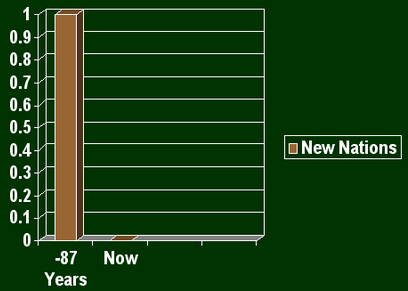
\includegraphics[width=0.5\textwidth]{gettysburg_graph}
\end{figure}

\begin{block}{Quatre fois vingt plus sept}
\begin{equation}
-(4 \times 20 + 7) = -87
\end{equation}
\end{block}

\end{frame}

\section{R�sum�}

\begin{frame}{R�sum�}

\begin{columns}
\begin{column}{0.4\textwidth}
\begin{itemize}
\item Nouvelle nation
\item Guerre civile
\item Terrain d�di�
\end{itemize}
\end{column}
\begin{column}{0.6\textwidth}
\begin{itemize}
\item D�dicace au travail non accompli
\item Nouvelle naissance de la libert�
\item Gouvernement non p�rissable
\end{itemize}
\end{column}
\end{columns}

\end{frame}

\end{document}

